%%% Title, author
%%% ------------------------------------------------------------	
\begin{center}
{\sffamily \begin{huge}\textbf{
	Utilização do PI SDK para criação de relatórios no Excel
	}\end{huge}\\[10pt]
{Hiuller C. Araujo}
}\\
	\begin{abstract}
	O objetivo deste trabalho é detalhar o desenvolvimento de um relatório em Excel com dados do PIMS recuperados via VBA e PI-SDK. O PI-SDK é uma ferramenta que permite a qualquer linguagem com suporte à programação COM acessar o banco de dados PIMS. O caso apresentado é o acompanhamento dos alarmes de transbordamento dos tanques das bombas saturadoras dos convertedores da Aciaria 2. O objetivo é acompanhar o número de alarmes e o tempo total entre duas datas informadas pelo usuário. 
	\end{abstract}
	\rule{4in}{0.5pt}
\end{center}
%%% Content
%%% ------------------------------------------------------------
\begin{multicols}{2}


\pagestyle{plain}
\setcounter{page}{1}
\pagenumbering{arabic}
% \thispagestyle{empty}
\section{Introdução}

	O PI-SDK (\emph{Software Development Kit}) é um controle ActiveX que provê acesso COM ao banco de dados do PIMS. O PI-SDK foi projetado para permitir fácil acesso aos dados do PIMS via Microsoft Visual Basic ou qualquer linguagem com suporte a programação COM\cite{pihelp}.
	
	A Figura \ref{fig:model} representa o modelo de objetos do PI-SDK. No topo, está a coleção de servidores \texttt{Servers}. Essa coleção guarda referências para os diferentes servidores. Cada servidor (\texttt{Server}) tem uma coleção de pontos (séries temporais) que são representados pela classe \texttt{PIPoint}. Cada \texttt{PIPoint} pode ser entendido como uma tag, na linguagem do \emph{PI ProcessBook}.
	\begin{figure}[H]
		\centering
		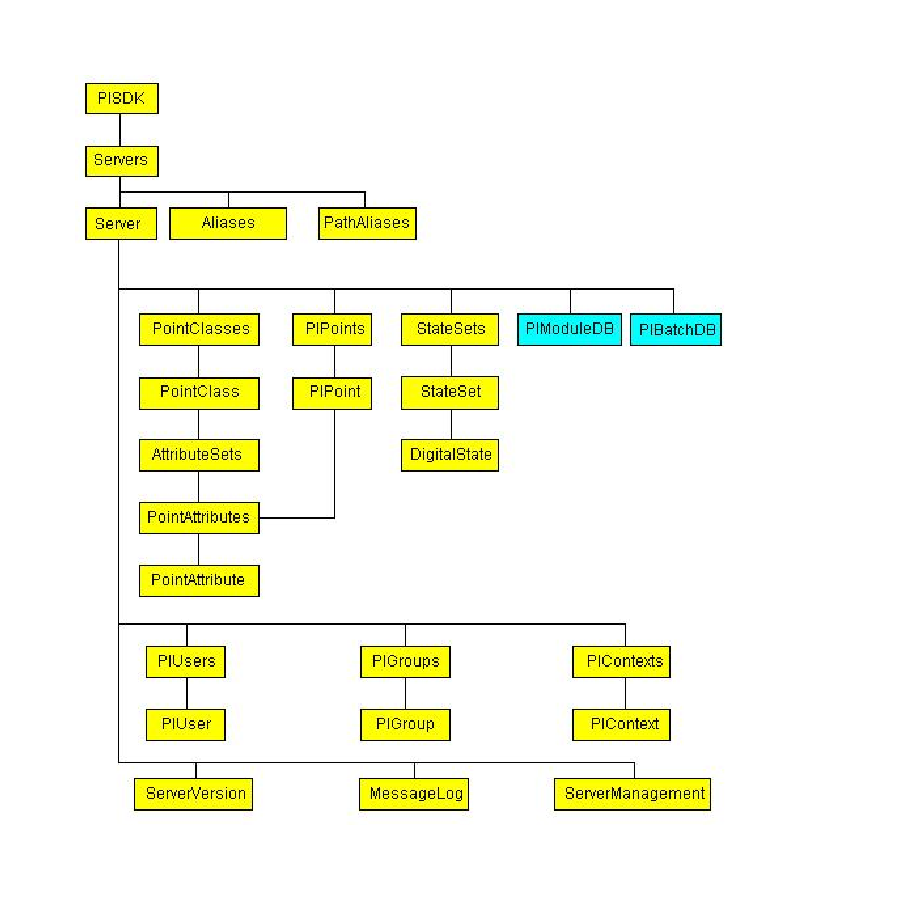
\includegraphics[scale=0.55, bb=0 0 432 432, trim=0in 0in 0in 0in]{figures/model.pdf} %left, bottom, right and top
		\caption{Modelo de objetos do PI-SDK\cite{pihelp}.}
		\label{fig:model}
	\end{figure}
	A estrutura do \texttt{PIPoint} tem um membro do tipo \texttt{Data} que fornece acesso aos dados na forma de um objeto \texttt{ADODB.Recordset}\cite{wiki:adors}, que é uma interface comum para forncer acesso a conjuntos de registros encontrada nos produtos do pacote \emph{Office} da Microsoft.
\section{Metodologia}
	Para a criação de um relatório com dados do PIMS, as principais etapas envolvidas são: a) obtenção dos dados numa estrutura manuseável e b) disposição gráfica dos valores. A obtenção dos dados foi implementada utilizando o conhecimento do modelo de objetos do PI-SDK para se obter um objeto \texttt{ADODB.Recordset} que é uma fonte de dados baseada em campos e valores que podem ser acessados sequencialmente. Para a apresentação gráfica dos resultados foram utilizadas técnicas triviais do ambiente Excel para criação de gráficos.
	
	A etapa de interesse para este trabalho refere-se à obtenção de dados do PIMS. Esta etapa foi dividida em duas fases de obtenção e leitura de um objeto \texttt{Recordset}.
\subsection{Obtenção do \texttt{Recordset}}
	A Figura \ref{fig:code} apresenta o código VBA desenvolvido para obtenção de dados de um servidor PIMS na forma de um objeto \texttt{Recordset}. O código declara objetos dos tipos do modelo de objetos do PI-SDK (vide Figura \ref{fig:model}). Para acessar estes tipos, o projeto VBA precisa fazer referência às bibliotecas \texttt{PISDK 1.3 Type Library} e \texttt{PISDK Commom 1.0 Type Library}.
	
	Ao objeto \texttt{Server} é atribuído o servidor padrão na linha 12 da Figura \ref{fig:code}. A linha 13 pega uma referência para a coleção de pontos do servidor padrão. A linha 14 seleciona um ponto específico pelo nome da tag, armazenado na \emph{array} \texttt{TagName} que tem valores para os convertedores 4 e 5. A linha 15 acessa o objeto \texttt{Data} do ponto e a linha 16 obtém um objeto do tipo \texttt{PIValue} entre as datas de inicio e fim. O método \texttt{RecordedValues} requer duas \emph{timestamps} que são \texttt{Variants} com o tipo \texttt{Date} do VBA. Na linha 17 é utilizado o método \texttt{Recordset} para obter um \texttt{ADODB.Recordset} do objeto \texttt{PIValues}.
	\begin{figure}[H]
		\centering
		\lstinputlisting[language=VBScript]{code/sample.vb}
		\caption{Código fonte utilizado para obtenção de um objeto \texttt{Recordset}.}
		\label{fig:code}
	\end{figure}			
\subsection{Leitura do \texttt{Recordset}}
	O \texttt{Recordset} é uma estrutura amigável para representar um conjunto de registros. Utiliza-se o método \texttt{MoveFirst} para ir para o primeiro registro e \texttt{MoveNext} para ir para o próximo registro. Para sinalizar o último registro existe o método \texttt{EOF} que retorna verdadeiro quando o fim da estrutura foi atingido. 
	
	A Figura \ref{fig:iterat} apresenta a estrutura de código utilizada para iteração sobre um \texttt{Recordset}. Depois de declarado e inicializado (linhas 1 e 2) o primeiro registro é acessado (linha 4). Enquanto o fim de estrutura não for atingido é feita a leitura e manipulação dos dados (linha 6). Depois, move-se para o próximo registro (linha 7).
	\begin{figure}[H]
		\centering
		\lstinputlisting[language=VBScript]{code/rs.vb}
		\caption{Modelo de iteração sobre \texttt{Recordset} em VBA.}
		\label{fig:iterat}
	\end{figure}			
	Os valores das diferentes colunas são acessados pela coleção \texttt{Fields} do \texttt{Recordset}. O PIMS retorna um \texttt{Recordset} com 
	Para o caso dos alarmes do tanque da saturadora, são utilizadas duas tags do PIMS que tem valor 1 quando o alarme está ativo e 0 caso contrário. O nome da tag foi armazenado num vetor do tipo \texttt{String} com dimensões 4 e 5 que correspondem aos convertedores.
	
	Os dados obtidos do PIMS contém uma lista de horários e os valores 1 que indicam que o instante de início do alarme e zero para insicar o instante de desligamento do alarme.
	\begin{figure}[H]
		\centering
		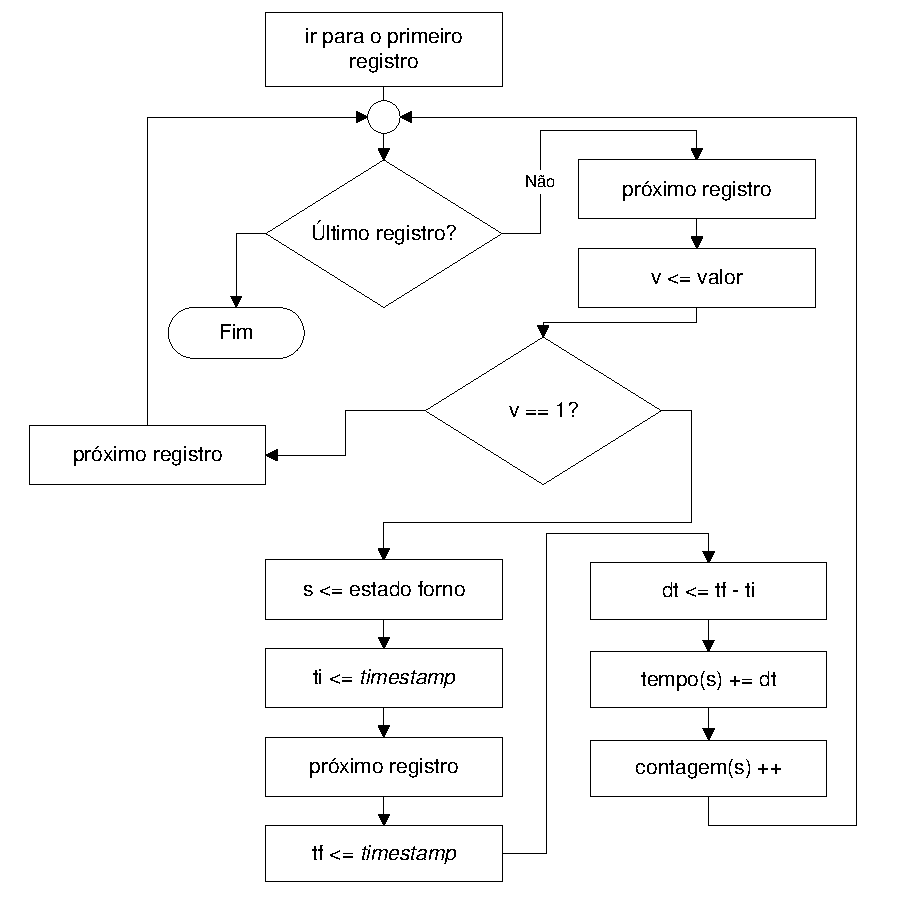
\includegraphics[scale=0.55, bb=0 0 432 432, trim=0in 0in 0in 0in]{figures/flux.pdf} %left, bottom, right and top
		\caption{Fluxograma utilizado para a contabilização do número de alarmes e da soma dos tempos.}
		\label{fig:alg}
	\end{figure}		
	
	
%%%%%%%%%%%%%%%%%%%%%%%%%%%%%%%%%%%%%%%%%%%%%%%%%%%%%%
\bibliographystyle{IEEE/abntex2-num}
% \bibliographystyle{IEEE/IEEEtranN}
% \bibliographystyle{plainnat}
% enable it only if you want to display some
% this command renames the reference section: http://tex.stackexchange.com/questions/12597/renaming-the-bibliography-page-using-bibtex
\renewcommand{\bibname}{Referências}
\bibliography{references}

\end{multicols}	